\chapter{ART Native Code Store}\label{chapter:native_code_store}

Since DEX code seems like to be the weak spot for Apps in terms of security
topics as well was for licensing and piracy issues, it seems logic to try
to circumvent this file format by design.
When comparing the mobile device distribution
system of Apps to desktop environments like Linux, Windows or MacOS, it becomes
clear that the main difference is the distribution of Java like byte-code compared to binaries, at least for commercial software or the operating system itself. So the question would be if it is possible to establish an App store that only distributes native code instead of APKs. Like deduced in \autoref{section:app_execution_detail}, it is more than very likely that the DEX file is still needed for addressing native code inside of an ELF.
Still that thought experiment will be performed in order to clarify if it is possible in general.

At first, an architecture needs to be defined that would be suitable for an alternative native code App store. To keep the user experience as is, it would be beneficial to be able to still use the Google Play App Store for distributing Apps. Therefore at least a bare-bone APK for the application needs to be created that will then be placed into the Google Store.
That application can then be installed the common Android way. At its first startup, it then could connect to the actual native code app store
requesting the functional App in form of raw byte code or an ELF file that
somehow gets injected in the current bare-bone application.
Since the Android ODEX ELF file of an App has the DEX embedded, it would need
to be adapted for instance leaving the DEX area blank.
So the skeleton version needs to implement at least the communication mechanism as well as the self modifying code part that can handle the receiving code snippets (\autoref{fig:native_store_arch} visually shows
the explained architecture).
\begin{figure}[htb]
  \centering
  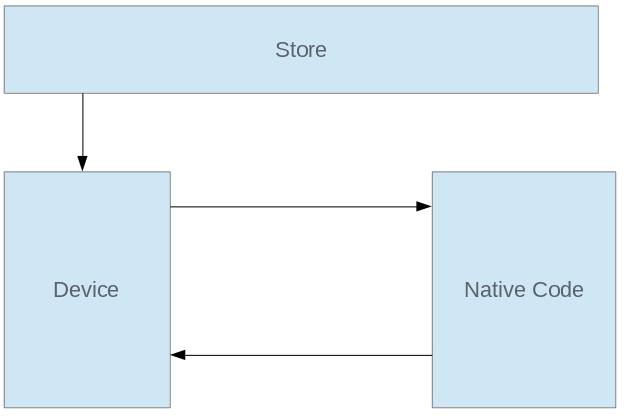
\includegraphics[scale=0.5]{figures/native_store_arch}
  \caption[Native Code Store Architecture]{Native Code Store Architecture}
  \label{fig:native_store_arch}
\end{figure}
When assuming that no root rights are present, the possibilities of injecting code and changing files are of course very limited. Remember that there do exist two identical DEX files after the installation process (post Android 5), one DEX inside of the original \code{base.apk} package and one embedded inside the \code{dex2oat} output (ELF file).
Let's see to whom those files belong at Linux layer and what permissions are set. Files stored at \code{/data/app} like the \code{base.apk}, the \code{lib/}
folder as well as \code{oat/} do belong to the \code{system} user. So accessing the \code{base.apk} container including its DEX should be
impossible out of the App context without root rights. Same goes for the
\code{base.odex} which also belongs to \code{system} and is marked as
``\code{rw-}''.
Another way to check the possibilities of changing files dynamically at runtime
are the mapped files and their permissions that can be read out of \code{/proc/self/maps} like explained in \autoref{section:memory_mapping} using C++.
Since the last entity of an App getting executed is the ODEX file, it is
mapped into the process (\autoref{tab:app_odex_mapping} shows an example)
\begin{table}[htb]
  \caption[App's ODEX/ELF mapping]{App's ODEX/ELF mapping}
  \label{tab:app_odex_mapping}
  %\centering
  \texttt{
  \begin{tabular}{l l l l l l}
    \toprule
    address & perms & offset & dev & inode & pathname \\
    \midrule
    a1d05000-a1fda000 & r--p & 00000000 & b3:1c & 171546 & /data/app/.../oat/arm/base.odex \\
    a1fda000-a22ab000 & r-xp & 002d5000 & b3:1c & 171546 & /data/app/.../oat/arm/base.odex \\
    a22ab000-a22ac000 & rw-p & 005a6000 & b3:1c & 171546 & /data/app/.../oat/arm/base.odex \\
    a22ac000-a2327000 & r--p & 006ed000 & b3:1c & 171546 & /data/app/.../oat/arm/base.odex \\
    \bottomrule
  \end{tabular}
  }
\end{table}
Several regions of the ODEX are mapped (offset marks the beginning relative to its file) with different permissions. Interesting is the part with writing permissions and its contents. The corresponding ELF format was analyzed in \autoref{section:elf_file_format}. To find out which specific section is mapped as writable, a program can be written in order to dump the content of every section including its offset or just using a hex editor. So first, the ODEX has to be pulled out of the Android device for which root rights are necessary. The file can then be moved into the \code{/sdcard} path and be pulled out using \code{adb pull /sdcard/base.odex} from a computer.
